\mychapter{1}{\textgamma+jet event classification in LHC collisions}
\label{chap:premierchapitre}

\section{CMS experiment at LHC}

The Compact Muon Solenoid (CMS) fig (\ref{cms}) is a particle physics detector built at one of the collision points of the Large Hadron Collider
(LHC) at CERN in switzerland and France. The goal of the CMS experiment is to investigate the physics of the Standard Model and beyond.
CMS is designed as a general-purpose detector, capable of studying many aspects of proton collisions at 0.9-13 TeV, the
center-of-mass energy range of the LHC particle accelerator.\\
CMS is made of multiple particle detectors designed to measure the energy and momentum of products of the collisions.
The innermost layer called the "Tracker" reconstruct the paths of charged particles comming from the collision or from the
decay of of short-lived particles.
%high-energy muons, electrons and hadrons as well as see
%tracks coming from the decay of very short-lived particles.\\
Next the "Electromagnetic Calorimeter" is designed to measure with high accuracy the energies of electrons and
photons.\\
The Hadronic Calorimeter measures the energy of hadrons.%and provides indirect measurement of the presence of
%non-interacting, uncharged particles such as neutrinos.\\
Theses layers all fit inside a large solenoid magnet of 3.8 Tesla, this allows the charge/mass ratio of particles to be
determined from the curved track that they follow in the magnetic field.
Finally the "Muon detectors and return yoke" are placed outside of the solenoid for detecting muons.

\begin{figure}[h!]
  \centering
  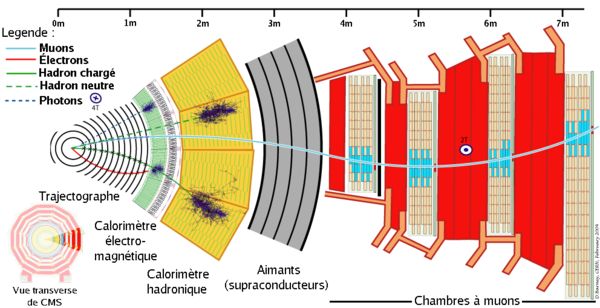
\includegraphics[width=0.8\textwidth]{cms}\\[1cm]
  \caption{Diagram of a slice of CMS detector, from left to right : tracker, electromagnetic calorimeter, hadronic
  calorimeter, superconductive solenoid and muon chamber. Lines represent track of particles.}
  \label{cms}
\end{figure}




\section{Hadronic jets in proton-proton collisions}

Jets are the experimental signatures of high-energy quarks and gluons produced in high-energy processes.\\
These particles having a colour charge, they cannot exist freely due to coulour-confinement, thereby they are not
directly observed in nature. Instead, they come together to form colour-neutral hadrons by a process called
hadronisation that leads to a collimated spray of hadrons called a jet.
The detailed understanding of both the jet transverse momentum and resolution is of crucial importance for many physics analyses.

%%% Local Variables: 
%%% mode: latex
%%% TeX-master: "isae-report-template"
%%% End: 
